\iffalse
\let\negmedspace\undefined
\let\negthickspace\undefined
\documentclass[journal,12pt,twocolumn]{IEEEtran}
\usepackage{cite}
\usepackage{amsmath,amssymb,amsfonts,amsthm}
\usepackage{algorithmic}
\usepackage{graphicx}
\usepackage{textcomp}
\usepackage{xcolor}
\usepackage{txfonts}
\usepackage{listings}
\usepackage{enumitem}
\usepackage{mathtools}
\usepackage{gensymb}
\usepackage{comment}
\usepackage[breaklinks=true]{hyperref}
\usepackage{tkz-euclide} 
\usepackage{listings}
\usepackage{gvv}                                        
\def\inputGnumericTable{}                                 
\usepackage[latin1]{inputenc}                                
\usepackage{color}                                            
\usepackage{array}                                            
\usepackage{longtable}                                       
\usepackage{calc}                                             
\usepackage{multirow}                                         
\usepackage{hhline}                                           
\usepackage{ifthen}                                           
\usepackage{lscape}

\newtheorem{theorem}{Theorem}[section]
\newtheorem{problem}{Problem}
\newtheorem{proposition}{Proposition}[section]
\newtheorem{lemma}{Lemma}[section]
\newtheorem{corollary}[theorem]{Corollary}
\newtheorem{example}{Example}[section]
\newtheorem{definition}[problem]{Definition}
\newcommand{\BEQA}{\begin{eqnarray}}
\newcommand{\EEQA}{\end{eqnarray}}
\newcommand{\define}{\stackrel{\triangle}{=}}
\theoremstyle{remark}
\newtheorem{rem}{Remark}
\begin{document}
\bibliographystyle{IEEEtran}
\vspace{3cm}
\title{\textbf{IN-2022}}
\author{EE23BTECH11210-Dhyana Teja Machineni$^{*}$% <-this % stops a space
}
\maketitle
\newpage
\bigskip

\textbf{QUESTION:}\\
A sinusoidal carrier wave with amplitude $A_c$ and frequency $f_c$ is amplitude modulated with a message signal $m\brak{t}$ having frequency $0 < f_m << f_c$ to generate the modulated wave $s\brak{t}$ given by
$s\brak{t}$ = $A_c\brak{1 + m\brak{t}}cos (2\pi f_c t)$
The message signal that can be retrieved completely using
envelope detection is \underline{{\hspace{1.5in}}}
\begin{enumerate}
    \item $m\brak{t}= 0.5 \cos{\brak{2 \pi f_m t}}$
    \item $m\brak{t}= 1.5 \sin{\brak{2 \pi f_m t}}$
    \item $m\brak{t}= 2 \sin{\brak{4 \pi f_m t}}$
    \item $m\brak{t}= 2 \cos{\brak{4 \pi f_m t}}$
\end{enumerate}
\solution
\fi
\begin{table}[h]
         \label{tab:table}
         \renewcommand{\arraystretch}{1.5}
\begin{tabular}{|c|c|}
\hline
Parameter & Description  \\\hline
$s\brak{t}$& Amplitude Modulated Wave \\\hline
$M\brak{t}$ & Message Signal \\\hline
$c\brak{t}$ & Carrier Signal \\\hline
$f_c$ & Frequency of Carrier Signal\\\hline
$f_m$& Frequency of Message Signal \\ \hline
\end{tabular}

         \caption{Variables and their descriptions}
     \end{table}\\
\begin{align}
c\brak{t}&=A_c \cos\brak{2 \pi f_c t}\\
   M\brak{t}&= A_m \cos\brak{2 \pi f_m t}\\
    s\brak{t}&= \brak{A_c+ M\brak{t}} \cos\brak{2\pi f_c t}\\
    &=A_c\brak{1+\frac{A_m}{A_c} \cos\brak{2 \pi f_m t}}\cos{2 \pi f_c t}\\
    &=A_c\brak{1+m\brak{t}}\cos{2 \pi f_c t}
\end{align}
Modulation Index of $s\brak{t}=\mu= \frac{A_m}{A_c}$
\begin{itemize}
    \item $\mu<1$  Signal is Can be detected
    \item $\mu=1$   Signal Cannot be detected
    \item $\mu>1$   Over modualtion 
\end{itemize}
\begin{enumerate}

    \item m\brak{t} = 0.5 cos\brak{2 \pi f_m t} 
\begin{align}
    \frac{A_m}{A_c}= 0.5 \\
    \mu <1
\end{align}
$\therefore$ Signal can be retrieved completely.
\renewcommand{\thefigure}{\theenumi}
 \renewcommand{\thetable}{\theenumi}
\begin{figure}[h]
  
  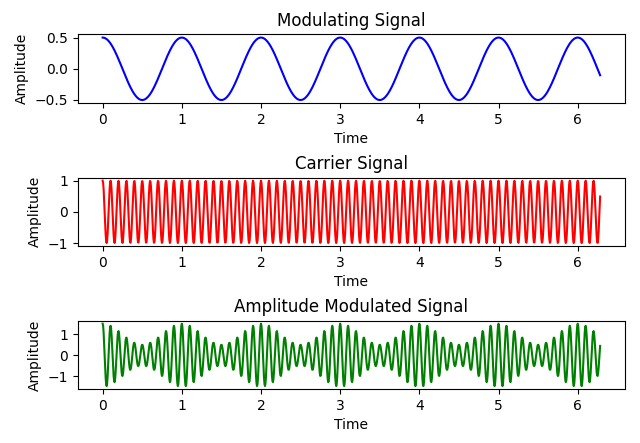
\includegraphics[width=\columnwidth]{2022/IN/16/figs/Figure_1.png}
  
\end{figure}
\item m\brak{t} = 1.5 sin\brak{2 \pi f_m t} 
\begin{align}
    \frac{A_m}{A_c}= 1.5\\
    \mu >1
\end{align}
$\therefore$ Signal cannot be retrieved completely.
\renewcommand{\thefigure}{\theenumi}
 \renewcommand{\thetable}{\theenumi}
\begin{figure}[h]
  
  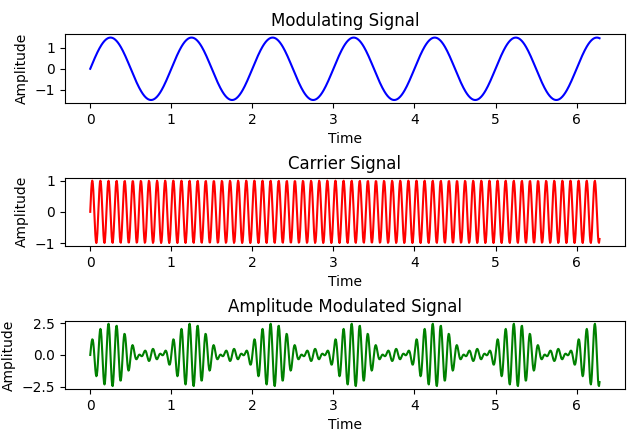
\includegraphics[width=\columnwidth]{2022/IN/16/figs/Figure_2.png}
  
\end{figure}
\item m\brak{t} = 2 sin\brak{4 \pi f_m t} 
\begin{align}
    \frac{A_m}{A_c}= 2\\
    \mu >1
\end{align}
$\therefore$ Signal cannot be retrieved completely.
\renewcommand{\thefigure}{\theenumi}
 \renewcommand{\thetable}{\theenumi}
\begin{figure}[h]
  
  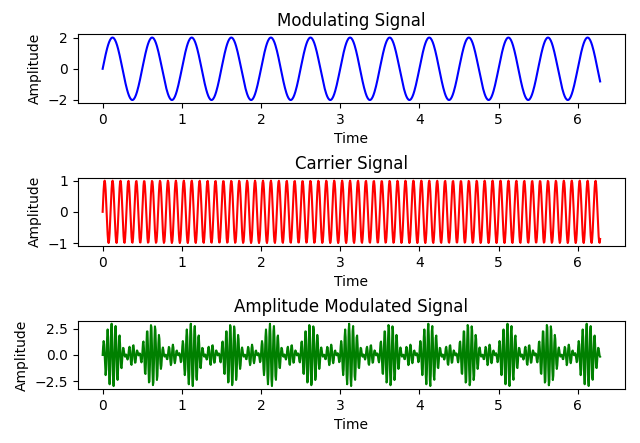
\includegraphics[width=\columnwidth]{2022/IN/16/figs/Figure_3.png}
  
\end{figure}
\item m\brak{t} = 2 cos\brak{4 \pi f_m t} 
\begin{align}
    \frac{A_m}{A_c}= 2\\
    \mu > 1
\end{align}
$\therefore$ Signal cannot be retrieved completely.
\renewcommand{\thefigure}{\theenumi}
 \renewcommand{\thetable}{\theenumi}
\begin{figure}[h]
  
  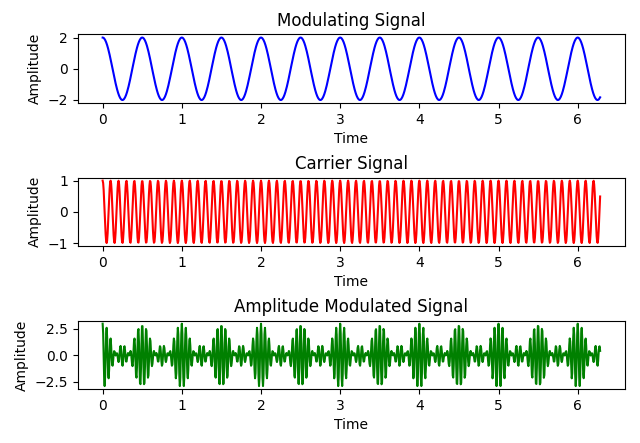
\includegraphics[width=\columnwidth]{2022/IN/16/figs/Figure_4.png}
  
\end{figure}
\end{enumerate}
 

